\documentclass[11pt]{article}

\usepackage[margin=1in]{geometry}
\usepackage{amsmath, amssymb}
\usepackage{graphicx}
\usepackage{hyperref}
\usepackage{enumitem}
\usepackage{xcolor}
\usepackage{float}
\usepackage{tikz}
\usetikzlibrary{arrows.meta, positioning}

\title{
    \normalsize IDs: 213851579, 213310485 \\[1em]
    \huge Video Processing -- Final Project \\
    \large Report
}

\author{}

\date{Course 0512.4263 \quad 2025/2026}

\begin{document}

\maketitle

% ========================================================================
\section*{Overview}
% ========================================================================

\noindent
The project processes a shaky video of a walking person in four stages. Each stage consumes the
previous stage's output:

\begin{figure}[H]
\centering
\resizebox{\textwidth}{!}{%
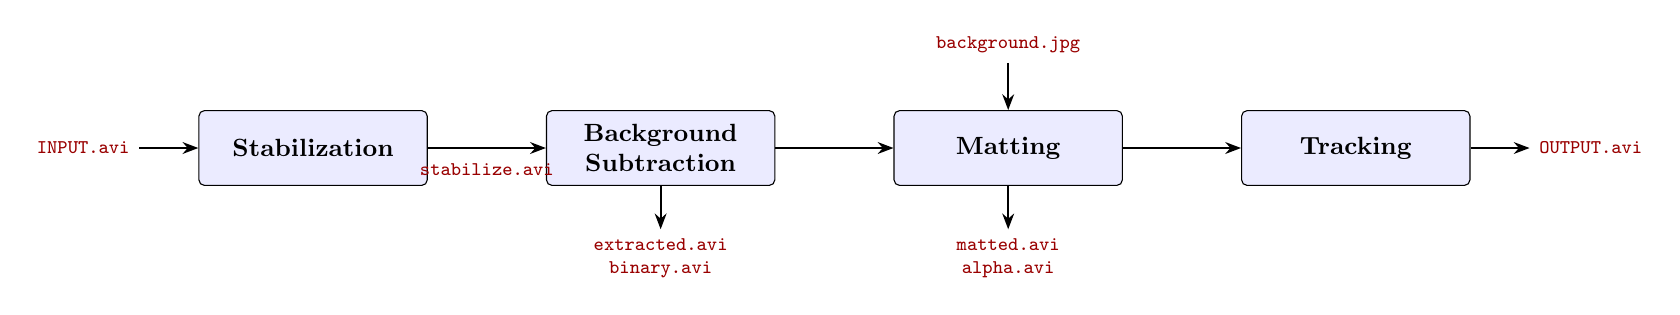
\begin{tikzpicture}[
    node distance=0.55cm and 1.5cm,
    stage/.style={draw, rounded corners=2pt, fill=blue!8, minimum width=2.9cm,
                  minimum height=0.95cm, font=\small\bfseries, align=center},
    art/.style={font=\scriptsize\ttfamily, text=red!60!black},
    arr/.style={-{Stealth[length=2mm]}, thick}
]
\node[stage] (stab) {Stabilization};
\node[stage, right=of stab] (bgs) {Background\\Subtraction};
\node[stage, right=of bgs] (mat) {Matting};
\node[stage, right=of mat] (trk) {Tracking};

\node[art, left=0.75cm of stab, align=center] (inp) {INPUT.avi};
\node[art, below=of bgs, align=center] (binext) {extracted.avi\\binary.avi};
\node[art, above=0.6cm of mat, align=center] (bg) {background.jpg};
\node[art, below=of mat, align=center] (matted) {matted.avi\\alpha.avi};
\node[art, right=0.75cm of trk, align=center] (outp) {OUTPUT.avi};

\draw[arr] (inp) -- (stab);
\draw[arr] (stab) -- node[art, below, yshift=-2pt] {stabilize.avi} (bgs);
\draw[arr] (bgs) -- (mat);
\draw[arr] (mat) -- (trk);
\draw[arr] (bgs) -- (binext);
\draw[arr] (bg) -- (mat);
\draw[arr] (mat) -- (matted);
\draw[arr] (trk) -- (outp);
\end{tikzpicture}%
}
\caption{The processing pipeline. Blue blocks are the implemented stages; red names are the
video/image artifacts each stage reads or writes.}
\end{figure}


% ========================================================================
\section{Stabilization}
% ========================================================================

\noindent
\textbf{Input.} \texttt{INPUT.avi} -- a shaky, handheld color video of a person walking.

\medskip
\noindent
\textbf{Expected output.} \texttt{stabilize\_ID1\_ID2.avi} -- the same video, in color, with the
camera motion cancelled: every frame is warped onto the coordinate system of the first frame, so
the background stays fixed for the next stage. Black regions near the frame borders are a known
side effect of the warp and are allowed.

\medskip
\noindent
\textbf{Algorithm.} We detect Shi--Tomasi corners and track them with pyramidal Lucas--Kanade
optical flow, both exactly as taught in the course (and implemented in Exercise 2; here we call
OpenCV's implementation for speed). A robust fit with RANSAC, also as seen in the lectures, maps
the tracked corners' positions onto a single global motion model per frame, and rejects the
corners that sit on the walking person, whose motion disagrees with the camera's. The frame is
then warped once, in color, by the fitted transform.

Two choices differ from the straightforward recipe and need a word:

\begin{itemize}[nosep]
    \item \emph{Anchored fit instead of composed transforms.} The usual approach estimates the
    motion from frame $t$ to $t-1$ and composes all these transforms to reach frame $0$. Composing
    $\sim$200 noisy estimates accumulates error, and the background slowly drifts. Instead, every
    tracked corner carries its frame-0 position (its ``anchor''), and each frame we fit the
    transform \emph{directly} from current positions to anchors. With no composition chain, drift
    cannot build up. Corners lost to occlusion or RANSAC rejection are replaced by freshly
    detected ones, anchored through the current fit.
    \item \emph{Homography as the motion model.} From the transformation ladder seen in class
    (translation $\to$ affine $\to$ homography) we use the homography. A handheld camera also
    rotates slightly out of the image plane, which creates a small perspective (keystone)
    distortion between frames; similarity and affine models cannot represent it, and with them a
    residual wobble remains visible.
\end{itemize}

\noindent
\textbf{Result.} In the output video the scene is static: walls, doors and posters stay in
place through the entire clip and only the person moves. Averaging all output frames gives a
sharp image of the corridor with a faint ghost of the walking person, which is exactly the
behaviour a stabilized static background should show. Narrow black wedges appear at the frame
borders, as expected.


% ========================================================================
\section{Background Subtraction}
% ========================================================================

\noindent
\textbf{Input.} \texttt{stabilize\_ID1\_ID2.avi} -- the stabilized color video from stage 1.

\medskip
\noindent
\textbf{Expected output.} Two videos: \texttt{extracted\_ID1\_ID2.avi}, where the person keeps
the original pixel values and everything else is black, and \texttt{binary\_ID1\_ID2.avi}, the
matching mask (person $=1$, saved scaled to 255).

\medskip
\noindent
\textbf{Algorithm.} The core is the per-pixel Gaussian Mixture Model background model from the
lectures, used as taught: each pixel holds $K=4$ Gaussians $(\mu_k, \sigma_k, \omega_k)$, a new
sample matches a Gaussian within $2.5\sigma$, matched Gaussians are updated and their weight
grows, unmatched ones decay, the weakest is replaced on no match, and the background Gaussians
are the top ones by $\omega_k/\sigma_k$ up to a cumulative weight $T = 0.7$, inside the lecture's
own suggested range of $0.7$--$0.9$. The departures from the lecture version:

\begin{itemize}[nosep]
    \item \emph{Offline instead of online.} The lecture's algorithm serves a live camera. We
    have the full video on disk, so the model is trained on the whole clip first and only then
    is every frame classified, against the final model.
    \item \emph{Median/MAD initialization.} The main Gaussian of every pixel starts at the
    pixel's temporal median color, with $\sigma$ from the median absolute deviation. The person
    covers any single pixel for a minority of the frames, so the median already \emph{is} the
    background; starting there instead of from a blind guess avoids pixels that never converge
    within the clip's length.
    \item \emph{CIE-Lab color space.} Matching runs in Lab with the illumination channel
    down-weighted: $d^2 = 0.25\,\Delta L^2 + \Delta a^2 + \Delta b^2$. Shadows and lighting
    changes live almost entirely in $L$, while the person differs in chroma, so this makes the
    classifier insensitive to illumination but sharp on real color change. A pixel whose $L$
    drops to 50--96\% of the background's while $a, b$ stay within 8 units is labelled a cast
    shadow and kept as background.
    \item \emph{Cleanup.} Morphological opening and closing (recommended in the lecture notes),
    keeping every connected component at least 20\% of the largest one (dark clothing can split
    a limb off the torso; keeping only the largest deletes real body parts), hole filling, and a
    smooth upscale of the mask back to full resolution.
\end{itemize}

\noindent
\textbf{Result.} The binary mask holds the complete silhouette -- head, arms, legs, shoes -- in
all frames, with no background patches, and the person's cast shadow on the floor is not
included. The extracted video shows the person cleanly cut out on black, with a smooth boundary,
ready for matting.


% ========================================================================
\section{Matting}
% ========================================================================

\noindent
\textbf{Input.} \textit{(to be completed)}

\medskip
\noindent
\textbf{Expected output.} \textit{(to be completed)}

\medskip
\noindent
\textbf{Algorithm.} \textit{(to be completed)}

\medskip
\noindent
\textbf{Result.} \textit{(to be completed)}


% ========================================================================
\section{Tracking}
% ========================================================================

\noindent
\textbf{Input.} \textit{(to be completed)}

\medskip
\noindent
\textbf{Expected output.} \textit{(to be completed)}

\medskip
\noindent
\textbf{Algorithm.} \textit{(to be completed)}

\medskip
\noindent
\textbf{Result.} \textit{(to be completed)}

\end{document}
